\clearpage

\section{Simulation Analysis}
\label{sec:simulation}

We started out by doing a simulation analysis of the circuit that was present above. The OP-AMP used is a subcircuit composed of of 2 capacitors, 5 diodes, a voltage-controled voltage source, a current-controlled current source, 2 voltage-controlled current sources, an independent current source, a current-controled voltage source, 2 transistors, 9 resistors and 6 independent voltage sources, making it an OP-AMP in the model uA741.

In Figure \ref{fig:sim-gain}, the result for the gain for various frequencies is presented.

\vspace{-3cm}

\begin{figure}[H] \centering
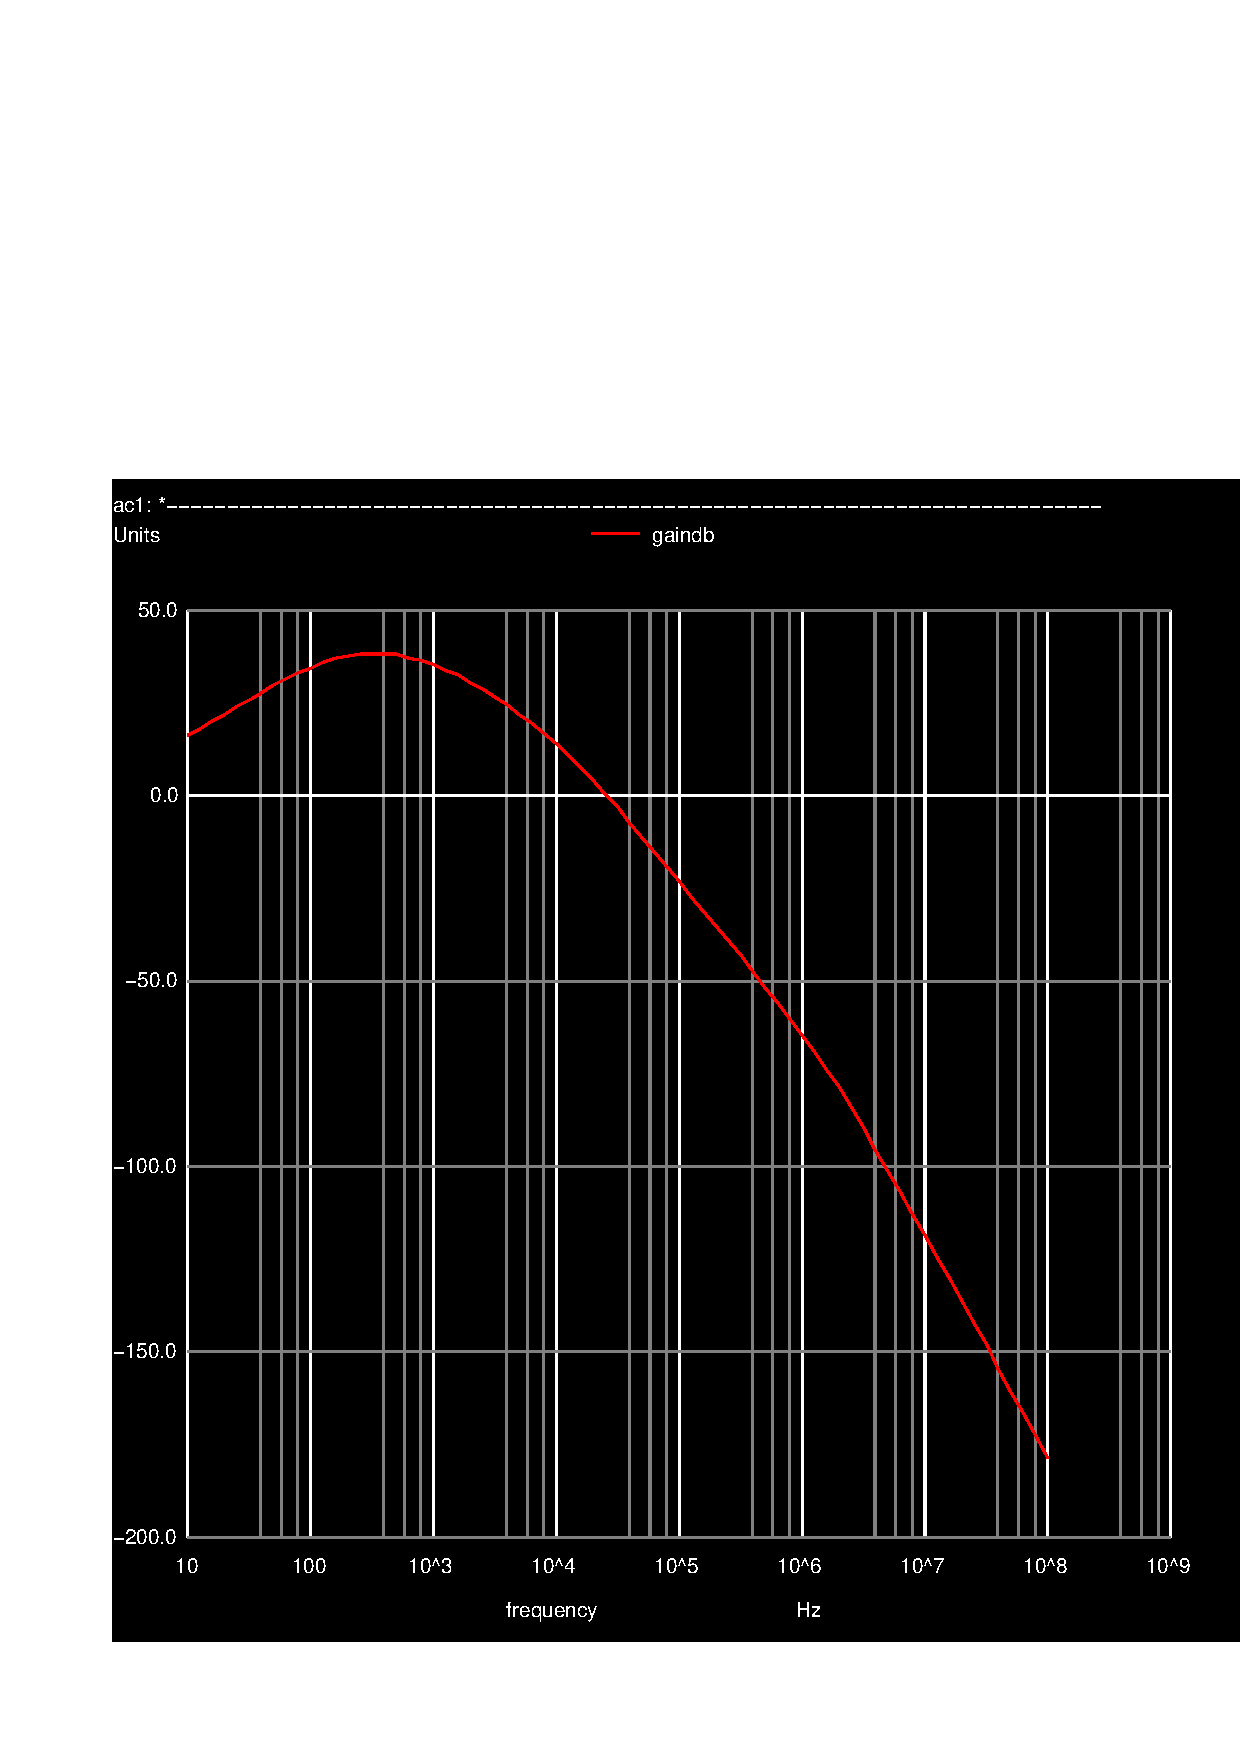
\includegraphics[width=0.5\linewidth]{../sim/gain.pdf}
\caption{Output Voltage Gain Simulated}
\label{fig:sim-gain}
\end{figure}

It is obvious that we were able to come quite close to the requested gain, but our central frequency is not the desired one. In the tables below the relevant results from the the graph in Figure \ref{fig:sim-gain} are presented, which lets us know that the higher cut-off frequency is actually very close to the desired central frequency, which means that our gain is still mostly relevant at 1000Hz.

\begin{center}
\begin{tabular}{|l|r|}
  \hline    
  {\bf Variable} & {\bf Value (dB)} \\ \hline
  gaindbmax & 3.834218e+01\\ \hline

  %\label{tab:gain-tab}
\end{tabular}
\end{center}

\begin{center}
\begin{tabular}{|l|r|}
  \hline    
  {\bf Variable} & {\bf Value (Hz)} \\ \hline
  f1 & 1.165730e+02\\ \hline
f2 & 9.936323e+02\\ \hline
bandwidth & 8.770593e+02\\ \hline
cenfreq & 3.403391e+02\\ \hline

 % \label{tab:freq-tab}
\end{tabular}
\end{center}

In Figure \ref{fig:sim-phase}, you are also able to see the phase of the circuit throughout the same range of frequencies.

\begin{figure}[H] \centering
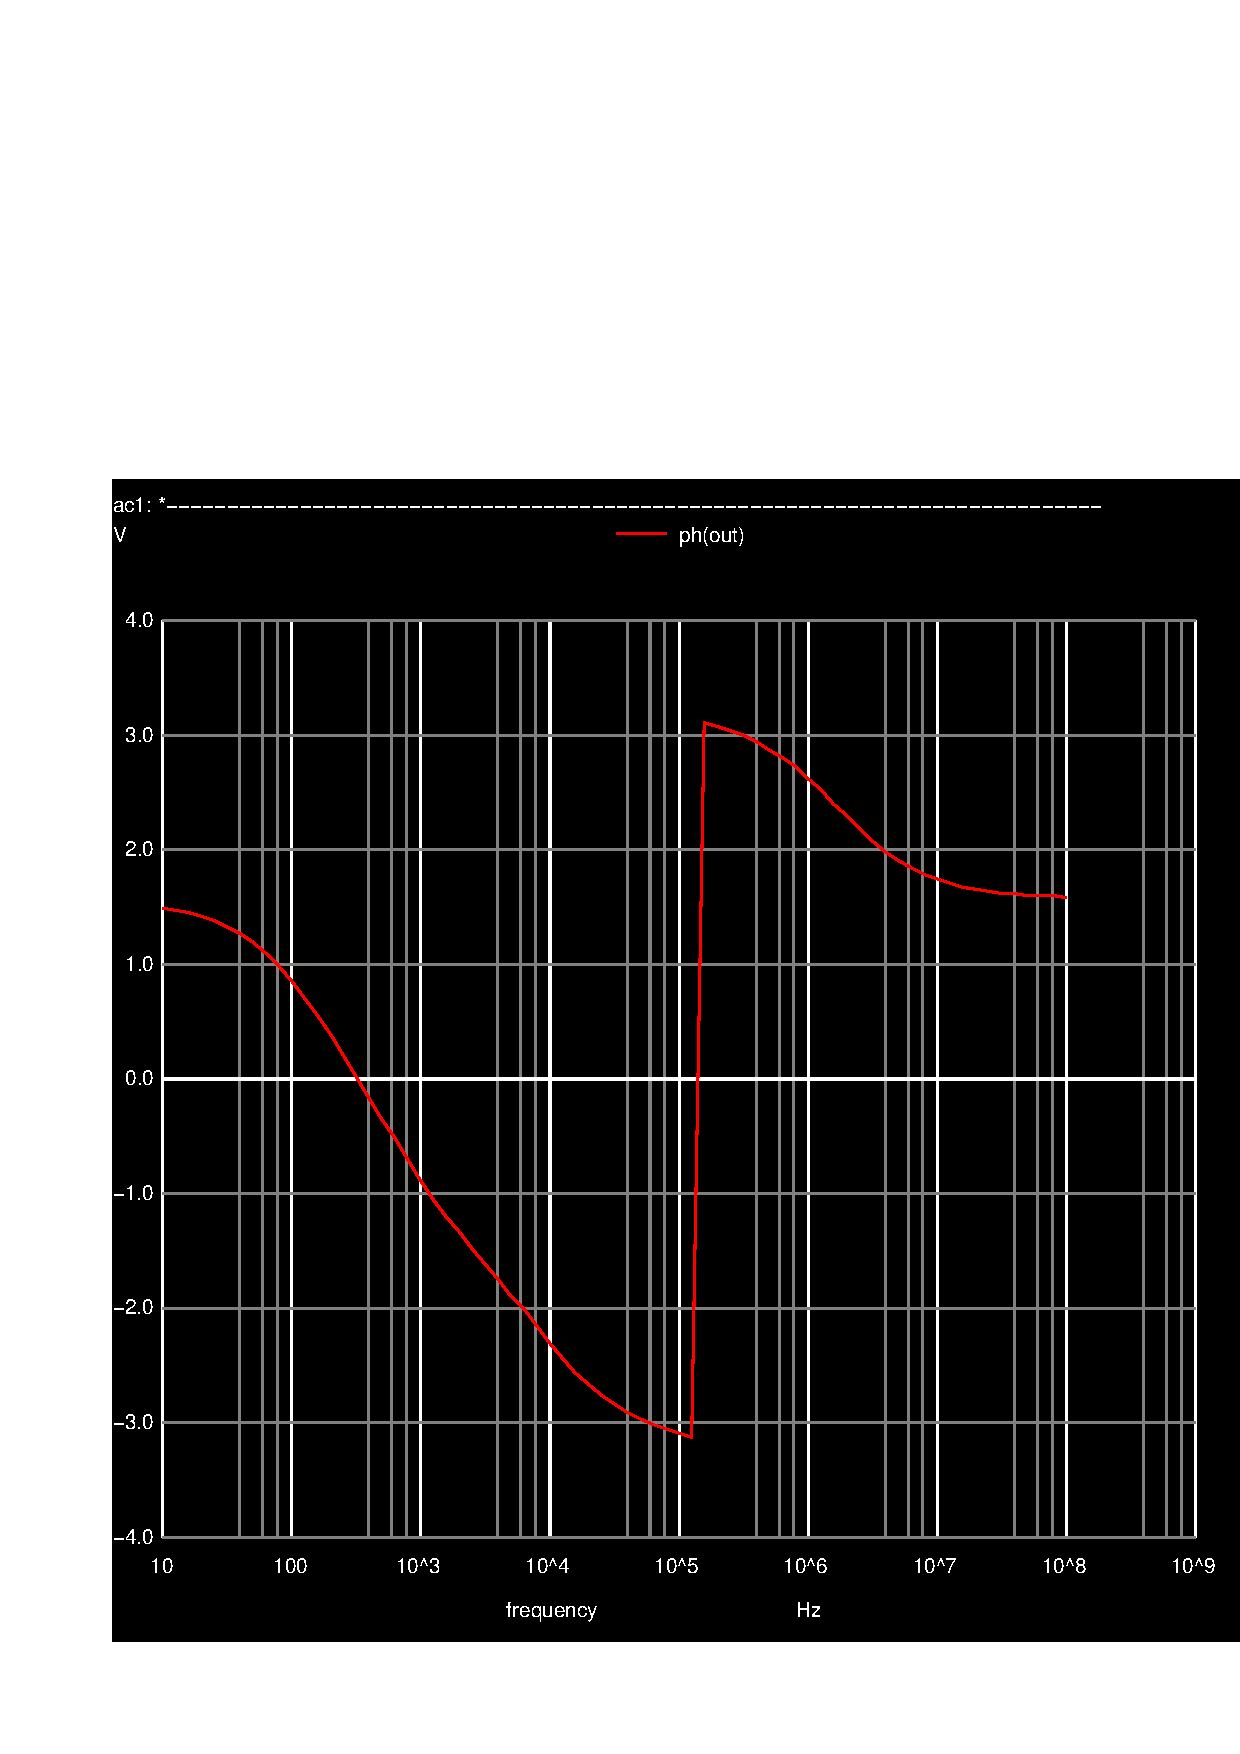
\includegraphics[width=0.5\linewidth]{../sim/phase.pdf}
\caption{Simulated Phase}
\label{fig:sim-phase}
\end{figure}

The discontinuance at around 10$^5$Hz is due to the fact that \textit{Ngspice}, the \textit{software} that was used for the simulation, automatically makes it so the values showed for the phase angle are between $\pi$ and -$\pi$, which lead to that. ESTAVA AQUI

\begin{center}
\begin{tabular}{|l|r|}
  \hline    
  {\bf Variable} & {\bf Value ($\Omega$)} \\ \hline
  zin & 9.999982e+02,-3.99820e+02\\ \hline

\end{tabular}
\end{center}


\subsection{Output Impedance Calculation}

For us to be able to calculate the output impedance, we had to create a new circuit, similar to the original one. However, in this new circuit, that is displayed in Figure \ref{fig:circuit-out}, we have turned off the input voltage source and substituted the load for that same source.

\begin{figure}[H] \centering
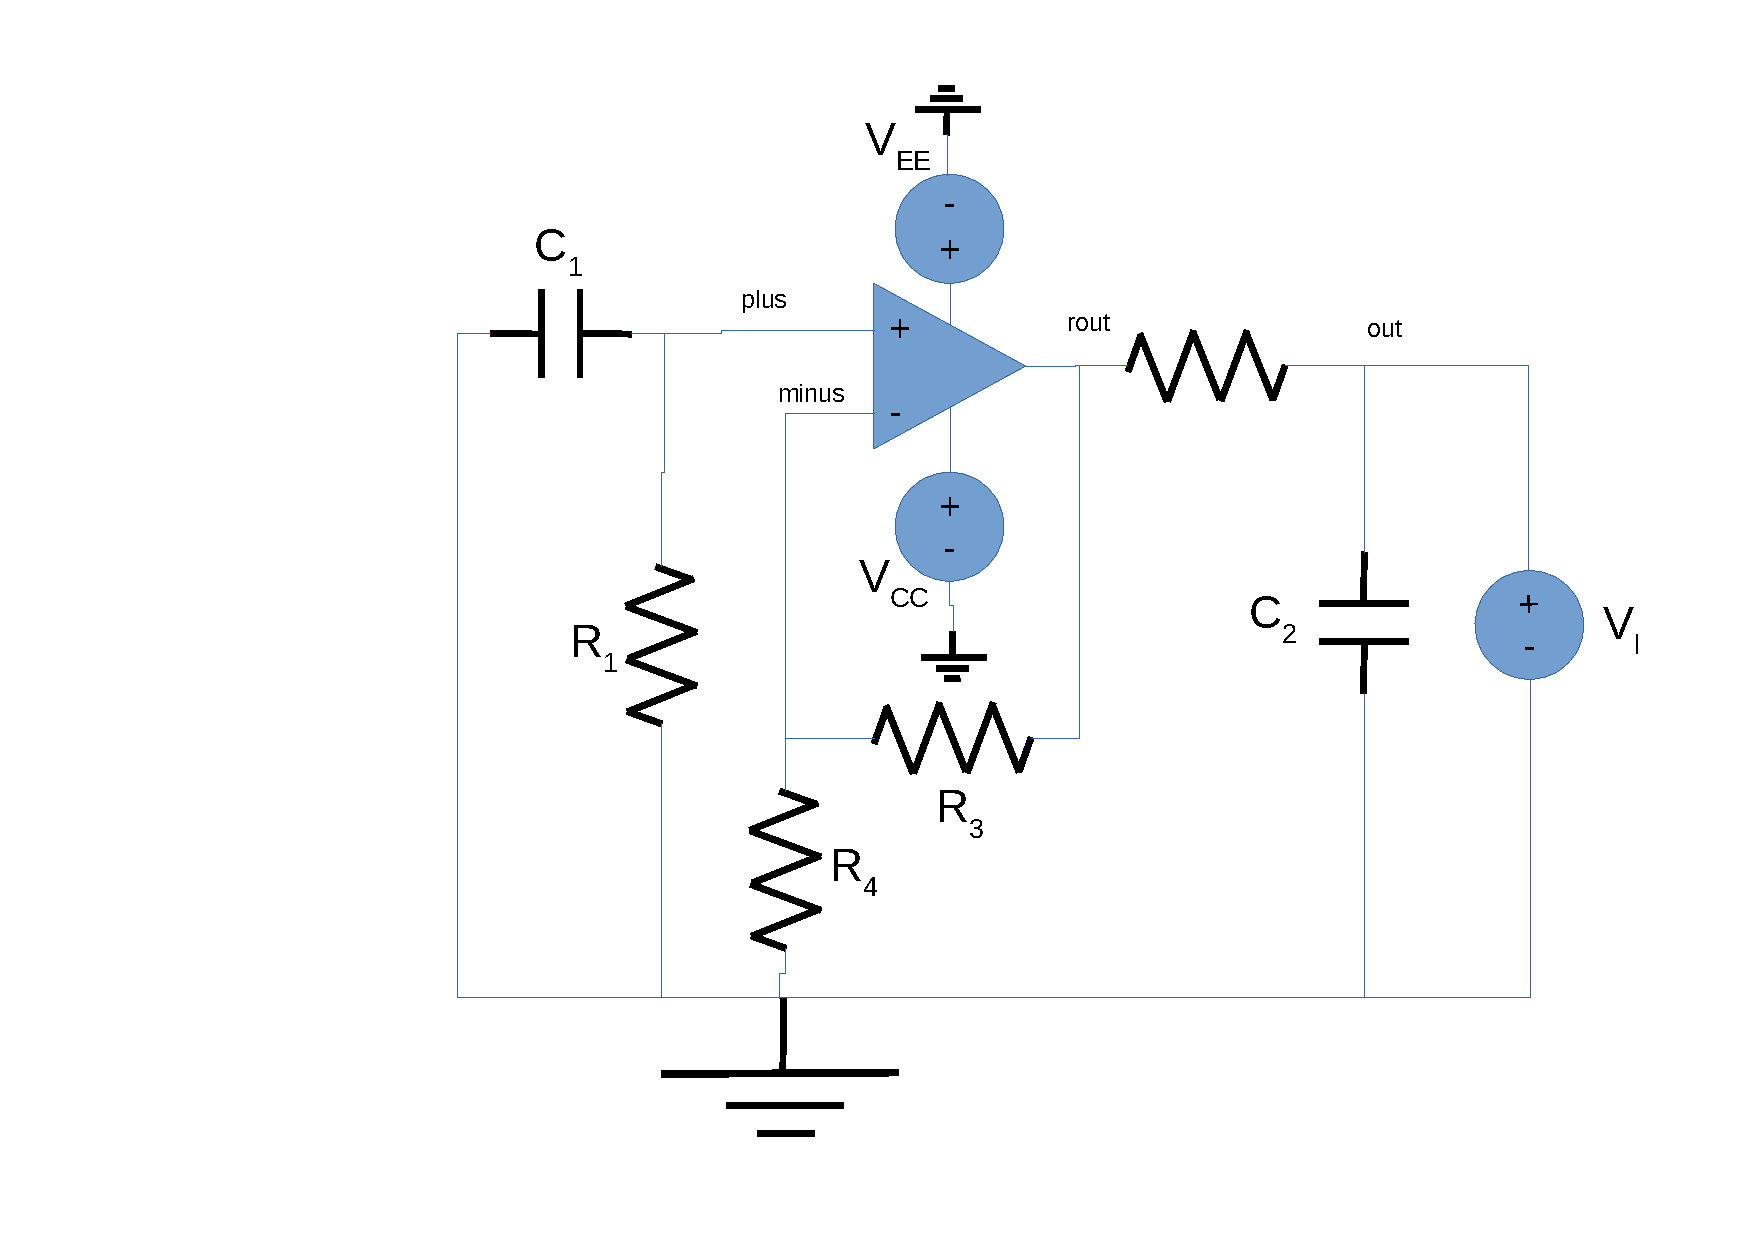
\includegraphics[width=0.7\linewidth]{circuit-out.pdf}
\caption{The circuit used to calculate the output impedance.}
\label{fig:circuit-out}
\end{figure}

\begin{center}
\begin{tabular}{|l|r|}
  \hline    
  {\bf Variable} & {\bf Value ($\Omega$)} \\ \hline
  zout & 8.011868e+02,-3.99270e+02\\ \hline

\end{tabular}
\end{center}

\begin{center}
\begin{tabular}{|l|r|}
  \hline    
  {\bf Variable} & {\bf Value (MU)} \\ \hline
  opampcost & 1.332329e+04\\ \hline
cost & 1.342749e+04\\ \hline

\end{tabular}
\end{center}

Relevant results:


\begin{center}
\begin{tabular}{|l|r|}
  \hline    
  {\bf Variable} & {\bf Value} \\ \hline
  merit & 5.223670e-02\\ \hline

\end{tabular}
\end{center}